\documentclass[12pt,]{book}
\usepackage{lmodern}
\usepackage{amssymb,amsmath}
\usepackage{ifxetex,ifluatex}
\usepackage{fixltx2e} % provides \textsubscript
\ifnum 0\ifxetex 1\fi\ifluatex 1\fi=0 % if pdftex
  \usepackage[T1]{fontenc}
  \usepackage[utf8]{inputenc}
\else % if luatex or xelatex
  \ifxetex
    \usepackage{mathspec}
  \else
    \usepackage{fontspec}
  \fi
  \defaultfontfeatures{Ligatures=TeX,Scale=MatchLowercase}
\fi
% use upquote if available, for straight quotes in verbatim environments
\IfFileExists{upquote.sty}{\usepackage{upquote}}{}
% use microtype if available
\IfFileExists{microtype.sty}{%
\usepackage{microtype}
\UseMicrotypeSet[protrusion]{basicmath} % disable protrusion for tt fonts
}{}
\usepackage[margin=1in]{geometry}
\usepackage{hyperref}
\hypersetup{unicode=true,
            pdftitle={ACC 471 - Final Report},
            pdfauthor={Jared Musil \& Jake McNair},
            pdfborder={0 0 0},
            breaklinks=true}
\urlstyle{same}  % don't use monospace font for urls
\usepackage{natbib}
\bibliographystyle{apalike}
\usepackage{color}
\usepackage{fancyvrb}
\newcommand{\VerbBar}{|}
\newcommand{\VERB}{\Verb[commandchars=\\\{\}]}
\DefineVerbatimEnvironment{Highlighting}{Verbatim}{commandchars=\\\{\}}
% Add ',fontsize=\small' for more characters per line
\usepackage{framed}
\definecolor{shadecolor}{RGB}{248,248,248}
\newenvironment{Shaded}{\begin{snugshade}}{\end{snugshade}}
\newcommand{\KeywordTok}[1]{\textcolor[rgb]{0.13,0.29,0.53}{\textbf{{#1}}}}
\newcommand{\DataTypeTok}[1]{\textcolor[rgb]{0.13,0.29,0.53}{{#1}}}
\newcommand{\DecValTok}[1]{\textcolor[rgb]{0.00,0.00,0.81}{{#1}}}
\newcommand{\BaseNTok}[1]{\textcolor[rgb]{0.00,0.00,0.81}{{#1}}}
\newcommand{\FloatTok}[1]{\textcolor[rgb]{0.00,0.00,0.81}{{#1}}}
\newcommand{\ConstantTok}[1]{\textcolor[rgb]{0.00,0.00,0.00}{{#1}}}
\newcommand{\CharTok}[1]{\textcolor[rgb]{0.31,0.60,0.02}{{#1}}}
\newcommand{\SpecialCharTok}[1]{\textcolor[rgb]{0.00,0.00,0.00}{{#1}}}
\newcommand{\StringTok}[1]{\textcolor[rgb]{0.31,0.60,0.02}{{#1}}}
\newcommand{\VerbatimStringTok}[1]{\textcolor[rgb]{0.31,0.60,0.02}{{#1}}}
\newcommand{\SpecialStringTok}[1]{\textcolor[rgb]{0.31,0.60,0.02}{{#1}}}
\newcommand{\ImportTok}[1]{{#1}}
\newcommand{\CommentTok}[1]{\textcolor[rgb]{0.56,0.35,0.01}{\textit{{#1}}}}
\newcommand{\DocumentationTok}[1]{\textcolor[rgb]{0.56,0.35,0.01}{\textbf{\textit{{#1}}}}}
\newcommand{\AnnotationTok}[1]{\textcolor[rgb]{0.56,0.35,0.01}{\textbf{\textit{{#1}}}}}
\newcommand{\CommentVarTok}[1]{\textcolor[rgb]{0.56,0.35,0.01}{\textbf{\textit{{#1}}}}}
\newcommand{\OtherTok}[1]{\textcolor[rgb]{0.56,0.35,0.01}{{#1}}}
\newcommand{\FunctionTok}[1]{\textcolor[rgb]{0.00,0.00,0.00}{{#1}}}
\newcommand{\VariableTok}[1]{\textcolor[rgb]{0.00,0.00,0.00}{{#1}}}
\newcommand{\ControlFlowTok}[1]{\textcolor[rgb]{0.13,0.29,0.53}{\textbf{{#1}}}}
\newcommand{\OperatorTok}[1]{\textcolor[rgb]{0.81,0.36,0.00}{\textbf{{#1}}}}
\newcommand{\BuiltInTok}[1]{{#1}}
\newcommand{\ExtensionTok}[1]{{#1}}
\newcommand{\PreprocessorTok}[1]{\textcolor[rgb]{0.56,0.35,0.01}{\textit{{#1}}}}
\newcommand{\AttributeTok}[1]{\textcolor[rgb]{0.77,0.63,0.00}{{#1}}}
\newcommand{\RegionMarkerTok}[1]{{#1}}
\newcommand{\InformationTok}[1]{\textcolor[rgb]{0.56,0.35,0.01}{\textbf{\textit{{#1}}}}}
\newcommand{\WarningTok}[1]{\textcolor[rgb]{0.56,0.35,0.01}{\textbf{\textit{{#1}}}}}
\newcommand{\AlertTok}[1]{\textcolor[rgb]{0.94,0.16,0.16}{{#1}}}
\newcommand{\ErrorTok}[1]{\textcolor[rgb]{0.64,0.00,0.00}{\textbf{{#1}}}}
\newcommand{\NormalTok}[1]{{#1}}
\usepackage{longtable,booktabs}
\usepackage{graphicx,grffile}
\makeatletter
\def\maxwidth{\ifdim\Gin@nat@width>\linewidth\linewidth\else\Gin@nat@width\fi}
\def\maxheight{\ifdim\Gin@nat@height>\textheight\textheight\else\Gin@nat@height\fi}
\makeatother
% Scale images if necessary, so that they will not overflow the page
% margins by default, and it is still possible to overwrite the defaults
% using explicit options in \includegraphics[width, height, ...]{}
\setkeys{Gin}{width=\maxwidth,height=\maxheight,keepaspectratio}
\IfFileExists{parskip.sty}{%
\usepackage{parskip}
}{% else
\setlength{\parindent}{0pt}
\setlength{\parskip}{6pt plus 2pt minus 1pt}
}
\setlength{\emergencystretch}{3em}  % prevent overfull lines
\providecommand{\tightlist}{%
  \setlength{\itemsep}{0pt}\setlength{\parskip}{0pt}}
\setcounter{secnumdepth}{5}
% Redefines (sub)paragraphs to behave more like sections
\ifx\paragraph\undefined\else
\let\oldparagraph\paragraph
\renewcommand{\paragraph}[1]{\oldparagraph{#1}\mbox{}}
\fi
\ifx\subparagraph\undefined\else
\let\oldsubparagraph\subparagraph
\renewcommand{\subparagraph}[1]{\oldsubparagraph{#1}\mbox{}}
\fi

%%% Use protect on footnotes to avoid problems with footnotes in titles
\let\rmarkdownfootnote\footnote%
\def\footnote{\protect\rmarkdownfootnote}

%%% Change title format to be more compact
\usepackage{titling}

% Create subtitle command for use in maketitle
\newcommand{\subtitle}[1]{
  \posttitle{
    \begin{center}\large#1\end{center}
    }
}

\setlength{\droptitle}{-2em}
  \title{ACC 471 - Final Report}
  \pretitle{\vspace{\droptitle}\centering\huge}
  \posttitle{\par}
\subtitle{Subtitle}
  \author{Jared Musil \& Jake McNair}
  \preauthor{\centering\large\emph}
  \postauthor{\par}
  \predate{\centering\large\emph}
  \postdate{\par}
  \date{2017-11-29}

\usepackage{booktabs}
\usepackage{amsthm}
\makeatletter
\def\thm@space@setup{%
  \thm@preskip=8pt plus 2pt minus 4pt
  \thm@postskip=\thm@preskip
}
\makeatother

\usepackage{amsthm}
\newtheorem{theorem}{Theorem}[chapter]
\newtheorem{lemma}{Lemma}[chapter]
\theoremstyle{definition}
\newtheorem{definition}{Definition}[chapter]
\newtheorem{corollary}{Corollary}[chapter]
\newtheorem{proposition}{Proposition}[chapter]
\theoremstyle{definition}
\newtheorem{example}{Example}[chapter]
\theoremstyle{remark}
\newtheorem*{remark}{Remark}
\begin{document}
\maketitle

{
\setcounter{tocdepth}{1}
\tableofcontents
}
\chapter{Prerequisites}\label{prerequisites}

\section{Foreword}\label{foreword}

This report was written using the R package \texttt{Bookdown}. This was
done as it allows for reproducable research of our data, methods, and
results. Where appropriate, the code has been included inline with the
results. All other methods are contained within the Appendix.

It is also available as a website reading on mobile devices, and and
epub for reading offline.

\section{Markdown Test}\label{markdown-test}

is a \emph{sample} book written in \textbf{Markdown}. You can use
anything that Pandoc's Markdown supports, e.g., a math equation
\(a^2 + b^2 = c^2\).

For now, you have to install the development versions of
\textbf{bookdown} from Github:

\begin{Shaded}
\begin{Highlighting}[]
\NormalTok{devtools::}\KeywordTok{install_github}\NormalTok{(}\StringTok{"rstudio/bookdown"}\NormalTok{)}
\end{Highlighting}
\end{Shaded}

Remember each Rmd file contains one and only one chapter, and a chapter
is defined by the first-level heading \texttt{\#}.

To compile this example to PDF, you need to install XeLaTeX.

\chapter{Introduction}\label{intro}

This

Throughout this report, the columns of our dataset will be refered to as
factors, and the rows of our dataset will be refered to as reccords.
This is to keep

\begin{center}\rule{0.5\linewidth}{\linethickness}\end{center}

You can label chapter and section titles using \texttt{\{\#label\}}
after them, e.g., we can reference Chapter \ref{intro}. If you do not
manually label them, there will be automatic labels anyway, e.g.,
Chapter \ref{methods}.

Figures and tables with captions will be placed in \texttt{figure} and
\texttt{table} environments, respectively.

\begin{Shaded}
\begin{Highlighting}[]
\KeywordTok{par}\NormalTok{(}\DataTypeTok{mar =} \KeywordTok{c}\NormalTok{(}\DecValTok{4}\NormalTok{, }\DecValTok{4}\NormalTok{, .}\DecValTok{1}\NormalTok{, .}\DecValTok{1}\NormalTok{))}
\KeywordTok{plot}\NormalTok{(pressure, }\DataTypeTok{type =} \StringTok{'b'}\NormalTok{, }\DataTypeTok{pch =} \DecValTok{19}\NormalTok{)}
\end{Highlighting}
\end{Shaded}

\begin{figure}

{\centering 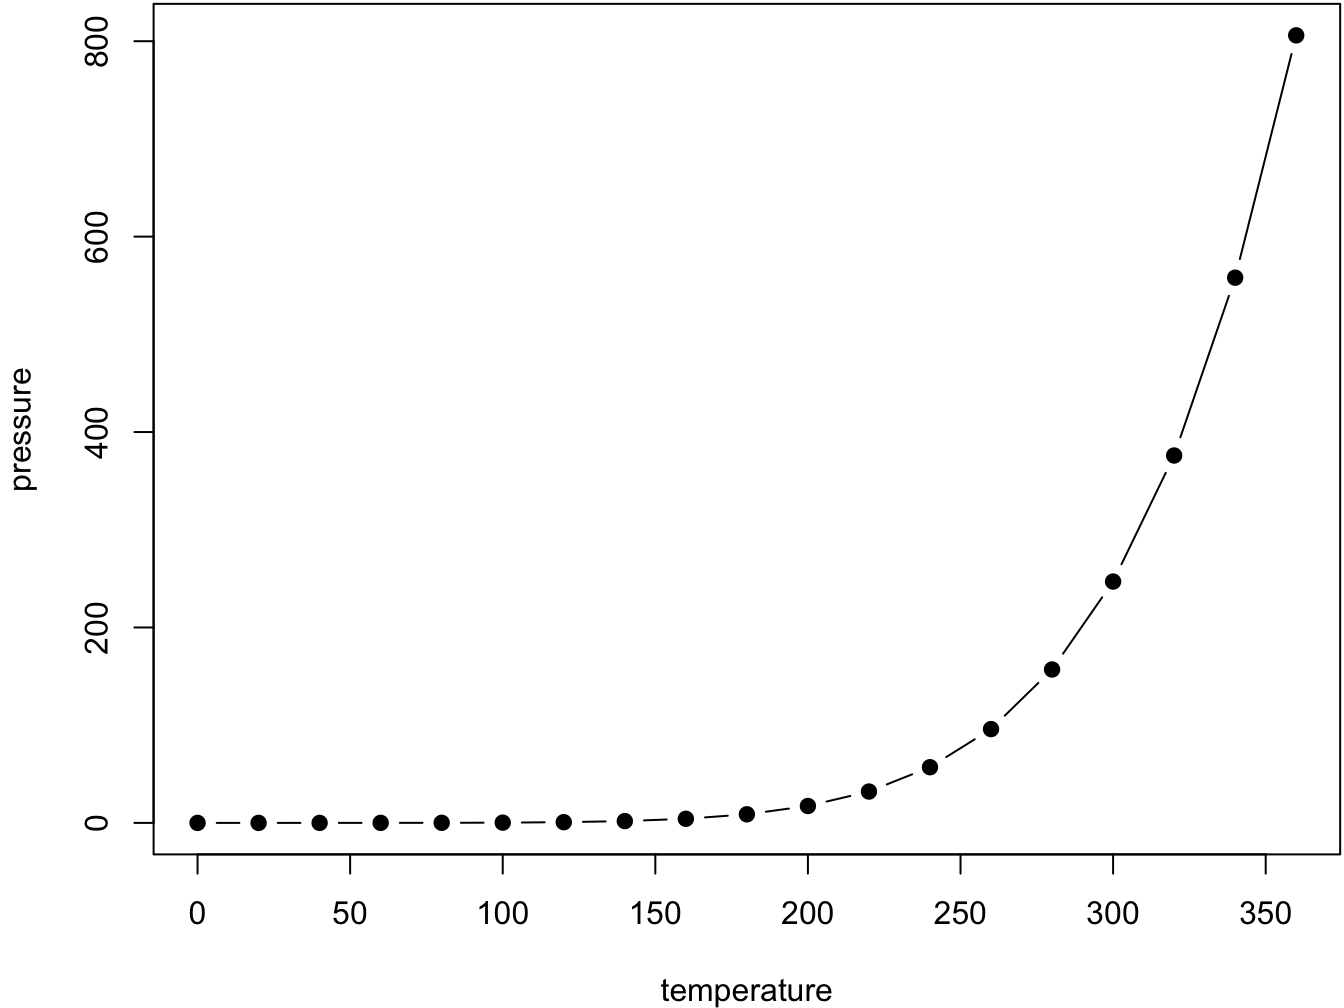
\includegraphics[width=0.8\linewidth]{bookdown-demo_files/figure-latex/nice-fig-1} 

}

\caption{Here is a nice figure!}\label{fig:nice-fig}
\end{figure}

Reference a figure by its code chunk label with the \texttt{fig:}
prefix, e.g., see Figure \ref{fig:nice-fig}. Similarly, you can
reference tables generated from \texttt{knitr::kable()}, e.g., see Table
\ref{tab:nice-tab}.

\begin{Shaded}
\begin{Highlighting}[]
\NormalTok{knitr::}\KeywordTok{kable}\NormalTok{(}
  \KeywordTok{head}\NormalTok{(iris, }\DecValTok{20}\NormalTok{), }\DataTypeTok{caption =} \StringTok{'Here is a nice table!'}\NormalTok{,}
  \DataTypeTok{booktabs =} \OtherTok{TRUE}
\NormalTok{)}
\end{Highlighting}
\end{Shaded}

\begin{table}

\caption{\label{tab:nice-tab}Here is a nice table!}
\centering
\begin{tabular}[t]{rrrrl}
\toprule
Sepal.Length & Sepal.Width & Petal.Length & Petal.Width & Species\\
\midrule
5.1 & 3.5 & 1.4 & 0.2 & setosa\\
4.9 & 3.0 & 1.4 & 0.2 & setosa\\
4.7 & 3.2 & 1.3 & 0.2 & setosa\\
4.6 & 3.1 & 1.5 & 0.2 & setosa\\
5.0 & 3.6 & 1.4 & 0.2 & setosa\\
\addlinespace
5.4 & 3.9 & 1.7 & 0.4 & setosa\\
4.6 & 3.4 & 1.4 & 0.3 & setosa\\
5.0 & 3.4 & 1.5 & 0.2 & setosa\\
4.4 & 2.9 & 1.4 & 0.2 & setosa\\
4.9 & 3.1 & 1.5 & 0.1 & setosa\\
\addlinespace
5.4 & 3.7 & 1.5 & 0.2 & setosa\\
4.8 & 3.4 & 1.6 & 0.2 & setosa\\
4.8 & 3.0 & 1.4 & 0.1 & setosa\\
4.3 & 3.0 & 1.1 & 0.1 & setosa\\
5.8 & 4.0 & 1.2 & 0.2 & setosa\\
\addlinespace
5.7 & 4.4 & 1.5 & 0.4 & setosa\\
5.4 & 3.9 & 1.3 & 0.4 & setosa\\
5.1 & 3.5 & 1.4 & 0.3 & setosa\\
5.7 & 3.8 & 1.7 & 0.3 & setosa\\
5.1 & 3.8 & 1.5 & 0.3 & setosa\\
\bottomrule
\end{tabular}
\end{table}

You can write citations, too. For example, we are using the
\textbf{bookdown} package \citep{R-bookdown} in this sample book, which
was built on top of R Markdown and \textbf{knitr} \citep{xie2015}.

\chapter{Problem Description}\label{problem-description}

The ability to utilize analytics to predict automobeile lossess is a
area of active research and application throughout the insurance and
fin-tech industries. All of the ``big four'' US domiciled auto insurrers
being State Farm, Geico, Allstate, and Progressive are actively engaging
in research to operationalize analytical models to increase operational
efficency. {[}citation needed\ldots{}{]}. This dataset is representitive
of claims data common to all of these auto insurance providers, and the
industry at large.

From a consumer standpoint, this has the potential to reduce average
claim times, reduce premium costs, and improve claims decisions (total
loss, not total loss).

\chapter{Data}\label{data}

Before doing any analysis, the feactors withing data set were first
checked for missing or invalid data. Of the original 205 reccords, 41
were removed because they contained missing data for the
\texttt{normalized-lossess} factor, which was coded as a \texttt{?}.
This resulted in a dataset of 164 reccords of clean data. No other
factors needed cleaning up, as the data was properly coded for each
reccord.

\begin{Shaded}
\begin{Highlighting}[]
\KeywordTok{library}\NormalTok{(readxl)}
\NormalTok{data_dict <-}\StringTok{ }\NormalTok{readxl::}\KeywordTok{read_xlsx}\NormalTok{(}\StringTok{"automobile-losses-data-dictionary.xlsx"}\NormalTok{)}
\NormalTok{knitr::}\KeywordTok{kable}\NormalTok{(}\KeywordTok{head}\NormalTok{(data_dict, }\DecValTok{20}\NormalTok{), }\DataTypeTok{caption =} \StringTok{'Data Dictionary - Initial'}\NormalTok{, }\DataTypeTok{booktabs =} \OtherTok{TRUE}\NormalTok{)}
\end{Highlighting}
\end{Shaded}

\begin{table}

\caption{\label{tab:data-dictionary}Data Dictionary - Initial}
\centering
\begin{tabular}[t]{rlll}
\toprule
\# & Description & Values & Keep\\
\midrule
1 & symboling & -3, -2, -1, 0, 1, 2, 3 & No\\
2 & normalized-losses & continuous from [65 to 256] & Yes\\
3 & make & alfa-romero, audi, bmw, chevrolet, dodge, honda, isuzu, jaguar, mazda, mercedes-benz, mercury, mitsubishi, nissan, peugot, plymouth, porsche, mitsubishi, nissan, peugot, plymouth, porsche, renault, saab, subaru, toyota, volkswagen, volvo & Yes\\
4 & fuel-type & diesel, gas & Yes\\
5 & aspiration & std, turbo & Yes\\
\addlinespace
6 & num-of-doors & four, two & Yes\\
7 & body-style & hardtop, wagon, sedan, hatchback, convertible & Yes\\
8 & drive-wheels & 4wd, fwd, rwd. & Yes\\
9 & engine-location & front, rear & Yes\\
10 & wheel-base & continuous from [86.6 to 120.9] & Yes\\
\addlinespace
11 & length & continuous from [141.1 to 208.1] & Yes\\
12 & width & continuous from [60.3 to 72.3] & Yes\\
13 & height & continuous from [47.8 to 59.8] & Yes\\
14 & curb-weight: & continuous from [1488 to 4066] & Yes\\
15 & engine-type & dohc, dohcv, l, ohc, ohcf, ohcv, rotor & Yes\\
\addlinespace
16 & num-of-cylinders & eight, five, four, six, three, twelve, two & Yes\\
17 & engine-size & continuous from [61 to 326] & Yes\\
18 & fuel-system & 1bbl, 2bbl, 4bbl, idi, mfi, mpfi, spdi, spfi & Yes\\
19 & bore & continuous from [2.54 to 3.94] & Yes\\
20 & stroke & continuous from [2.07 to 4.17] & Yes\\
\bottomrule
\end{tabular}
\end{table}

Of these factors, 10 of the initial 26 were removed, resulting in the 16
factors that will be used in analysis. These factors are noted in green
in \texttt{Keep} column of the above table.

The objective factor in the dataset is determined to be ``.

Next, the data was partitioned into three groups named \emph{training},
\emph{test}, and \emph{validation}. This was

\begin{Shaded}
\begin{Highlighting}[]
\NormalTok{data <-}\StringTok{ }\NormalTok{readxl::}\KeywordTok{read_xlsx}\NormalTok{(}\StringTok{"automobile-losses.xlsx"}\NormalTok{)}
\NormalTok{knitr::}\KeywordTok{kable}\NormalTok{(}\KeywordTok{head}\NormalTok{(data, }\DecValTok{20}\NormalTok{), }\DataTypeTok{caption =} \StringTok{'Dataset'}\NormalTok{, }\DataTypeTok{booktabs =} \OtherTok{TRUE}\NormalTok{)}
\end{Highlighting}
\end{Shaded}

\begin{table}

\caption{\label{tab:raw-data}Dataset}
\centering
\begin{tabular}[t]{rllllllllrrrrrllrlllrllrrl}
\toprule
1 & 2 & 3 & 4 & 5 & 6 & 7 & 8 & 9 & 10 & 11 & 12 & 13 & 14 & 15 & 16 & 17 & 18 & 19 & 20 & 21 & 22 & 23 & 24 & 25 & 26\\
\midrule
3 & ? & alfa-romero & gas & std & two & convertible & rwd & front & 88.6 & 168.8 & 64.1 & 48.8 & 2548 & dohc & four & 130 & mpfi & 3.47 & 2.68 & 9.0 & 111 & 5000 & 21 & 27 & 13495\\
3 & ? & alfa-romero & gas & std & two & convertible & rwd & front & 88.6 & 168.8 & 64.1 & 48.8 & 2548 & dohc & four & 130 & mpfi & 3.47 & 2.68 & 9.0 & 111 & 5000 & 21 & 27 & 16500\\
1 & ? & alfa-romero & gas & std & two & hatchback & rwd & front & 94.5 & 171.2 & 65.5 & 52.4 & 2823 & ohcv & six & 152 & mpfi & 2.68 & 3.47 & 9.0 & 154 & 5000 & 19 & 26 & 16500\\
2 & 164 & audi & gas & std & four & sedan & fwd & front & 99.8 & 176.6 & 66.2 & 54.3 & 2337 & ohc & four & 109 & mpfi & 3.19 & 3.4 & 10.0 & 102 & 5500 & 24 & 30 & 13950\\
2 & 164 & audi & gas & std & four & sedan & 4wd & front & 99.4 & 176.6 & 66.4 & 54.3 & 2824 & ohc & five & 136 & mpfi & 3.19 & 3.4 & 8.0 & 115 & 5500 & 18 & 22 & 17450\\
\addlinespace
2 & ? & audi & gas & std & two & sedan & fwd & front & 99.8 & 177.3 & 66.3 & 53.1 & 2507 & ohc & five & 136 & mpfi & 3.19 & 3.4 & 8.5 & 110 & 5500 & 19 & 25 & 15250\\
1 & 158 & audi & gas & std & four & sedan & fwd & front & 105.8 & 192.7 & 71.4 & 55.7 & 2844 & ohc & five & 136 & mpfi & 3.19 & 3.4 & 8.5 & 110 & 5500 & 19 & 25 & 17710\\
1 & ? & audi & gas & std & four & wagon & fwd & front & 105.8 & 192.7 & 71.4 & 55.7 & 2954 & ohc & five & 136 & mpfi & 3.19 & 3.4 & 8.5 & 110 & 5500 & 19 & 25 & 18920\\
1 & 158 & audi & gas & turbo & four & sedan & fwd & front & 105.8 & 192.7 & 71.4 & 55.9 & 3086 & ohc & five & 131 & mpfi & 3.13 & 3.4 & 8.3 & 140 & 5500 & 17 & 20 & 23875\\
0 & ? & audi & gas & turbo & two & hatchback & 4wd & front & 99.5 & 178.2 & 67.9 & 52.0 & 3053 & ohc & five & 131 & mpfi & 3.13 & 3.4 & 7.0 & 160 & 5500 & 16 & 22 & ?\\
\addlinespace
2 & 192 & bmw & gas & std & two & sedan & rwd & front & 101.2 & 176.8 & 64.8 & 54.3 & 2395 & ohc & four & 108 & mpfi & 3.5 & 2.8 & 8.8 & 101 & 5800 & 23 & 29 & 16430\\
0 & 192 & bmw & gas & std & four & sedan & rwd & front & 101.2 & 176.8 & 64.8 & 54.3 & 2395 & ohc & four & 108 & mpfi & 3.5 & 2.8 & 8.8 & 101 & 5800 & 23 & 29 & 16925\\
0 & 188 & bmw & gas & std & two & sedan & rwd & front & 101.2 & 176.8 & 64.8 & 54.3 & 2710 & ohc & six & 164 & mpfi & 3.31 & 3.19 & 9.0 & 121 & 4250 & 21 & 28 & 20970\\
0 & 188 & bmw & gas & std & four & sedan & rwd & front & 101.2 & 176.8 & 64.8 & 54.3 & 2765 & ohc & six & 164 & mpfi & 3.31 & 3.19 & 9.0 & 121 & 4250 & 21 & 28 & 21105\\
1 & ? & bmw & gas & std & four & sedan & rwd & front & 103.5 & 189.0 & 66.9 & 55.7 & 3055 & ohc & six & 164 & mpfi & 3.31 & 3.19 & 9.0 & 121 & 4250 & 20 & 25 & 24565\\
\addlinespace
0 & ? & bmw & gas & std & four & sedan & rwd & front & 103.5 & 189.0 & 66.9 & 55.7 & 3230 & ohc & six & 209 & mpfi & 3.62 & 3.39 & 8.0 & 182 & 5400 & 16 & 22 & 30760\\
0 & ? & bmw & gas & std & two & sedan & rwd & front & 103.5 & 193.8 & 67.9 & 53.7 & 3380 & ohc & six & 209 & mpfi & 3.62 & 3.39 & 8.0 & 182 & 5400 & 16 & 22 & 41315\\
0 & ? & bmw & gas & std & four & sedan & rwd & front & 110.0 & 197.0 & 70.9 & 56.3 & 3505 & ohc & six & 209 & mpfi & 3.62 & 3.39 & 8.0 & 182 & 5400 & 15 & 20 & 36880\\
2 & 121 & chevrolet & gas & std & two & hatchback & fwd & front & 88.4 & 141.1 & 60.3 & 53.2 & 1488 & l & three & 61 & 2bbl & 2.91 & 3.03 & 9.5 & 48 & 5100 & 47 & 53 & 5151\\
1 & 98 & chevrolet & gas & std & two & hatchback & fwd & front & 94.5 & 155.9 & 63.6 & 52.0 & 1874 & ohc & four & 90 & 2bbl & 3.03 & 3.11 & 9.6 & 70 & 5400 & 38 & 43 & 6295\\
\bottomrule
\end{tabular}
\end{table}

\begin{Shaded}
\begin{Highlighting}[]
\NormalTok{data <-}\StringTok{ }\NormalTok{readxl::}\KeywordTok{read_xlsx}\NormalTok{(}\StringTok{"automobile-losses.xlsx"}\NormalTok{)}
\KeywordTok{summary}\NormalTok{(data)}
\end{Highlighting}
\end{Shaded}

\begin{verbatim}
##        1                2                  3            
##  Min.   :-2.0000   Length:205         Length:205        
##  1st Qu.: 0.0000   Class :character   Class :character  
##  Median : 1.0000   Mode  :character   Mode  :character  
##  Mean   : 0.8341                                        
##  3rd Qu.: 2.0000                                        
##  Max.   : 3.0000                                        
##       4                  5                  6            
##  Length:205         Length:205         Length:205        
##  Class :character   Class :character   Class :character  
##  Mode  :character   Mode  :character   Mode  :character  
##                                                          
##                                                          
##                                                          
##       7                  8                  9                   10        
##  Length:205         Length:205         Length:205         Min.   : 86.60  
##  Class :character   Class :character   Class :character   1st Qu.: 94.50  
##  Mode  :character   Mode  :character   Mode  :character   Median : 97.00  
##                                                           Mean   : 98.76  
##                                                           3rd Qu.:102.40  
##                                                           Max.   :120.90  
##        11              12              13              14      
##  Min.   :141.1   Min.   :60.30   Min.   :47.80   Min.   :1488  
##  1st Qu.:166.3   1st Qu.:64.10   1st Qu.:52.00   1st Qu.:2145  
##  Median :173.2   Median :65.50   Median :54.10   Median :2414  
##  Mean   :174.0   Mean   :65.91   Mean   :53.72   Mean   :2556  
##  3rd Qu.:183.1   3rd Qu.:66.90   3rd Qu.:55.50   3rd Qu.:2935  
##  Max.   :208.1   Max.   :72.30   Max.   :59.80   Max.   :4066  
##       15                 16                  17             18           
##  Length:205         Length:205         Min.   : 61.0   Length:205        
##  Class :character   Class :character   1st Qu.: 97.0   Class :character  
##  Mode  :character   Mode  :character   Median :120.0   Mode  :character  
##                                        Mean   :126.9                     
##                                        3rd Qu.:141.0                     
##                                        Max.   :326.0                     
##       19                 20                  21             22           
##  Length:205         Length:205         Min.   : 7.00   Length:205        
##  Class :character   Class :character   1st Qu.: 8.60   Class :character  
##  Mode  :character   Mode  :character   Median : 9.00   Mode  :character  
##                                        Mean   :10.14                     
##                                        3rd Qu.: 9.40                     
##                                        Max.   :23.00                     
##       23                  24              25             26           
##  Length:205         Min.   :13.00   Min.   :16.00   Length:205        
##  Class :character   1st Qu.:19.00   1st Qu.:25.00   Class :character  
##  Mode  :character   Median :24.00   Median :30.00   Mode  :character  
##                     Mean   :25.22   Mean   :30.75                     
##                     3rd Qu.:30.00   3rd Qu.:34.00                     
##                     Max.   :49.00   Max.   :54.00
\end{verbatim}

\chapter{Methods Used}\label{methods-used}

We utilized \texttt{X} methods in our analysis, while settlling on
regression trees for our final reccomendations.

\chapter{Results}\label{results}

\ldots{}

\section{Example one}\label{example-one}

\section{Example two}\label{example-two}

\chapter{Reccomentations}\label{reccomentations}

\ldots{}

\chapter{Future Analysis}\label{future-analysis}

\ldots{}

\chapter{Conculsion}\label{conculsion}

\ldots{}

\bibliography{packages.bib,book.bib}


\end{document}
